\chapter{Implementation}
\label{chapter:implementation}

The actual implementation of the designed algorithms introduced in Chapter~\ref{chapter:methods} is now extensively described. 
As anticipated in the previous Chapter, here all the details of the developed phases of the project are deeply analysed and explained. 
A path similar to the one followed during the actual designing of the algorithms is used for outlining the whole project.\\
First of all, the preparatory tests performed for evaluating the feasibility of the conceived idea are reported and explained. 
Subsequently, the focus moves on the two main methods designed, the derivative based one and the strategy based on the standard SGM pipeline.
After that, the side phases of the work are presented. 
The pre and post-processing operations are accurately defined and the comparison among the different filtering operations are carried out.

\section{Preparatory and testing phase on MATLAB}
\label{section:prep-pahse-matlab}

\begin{figure}[t]
	\centering
	\subfigure[Left ground truth stereo test image overlapped by a simulated point grid]{
 		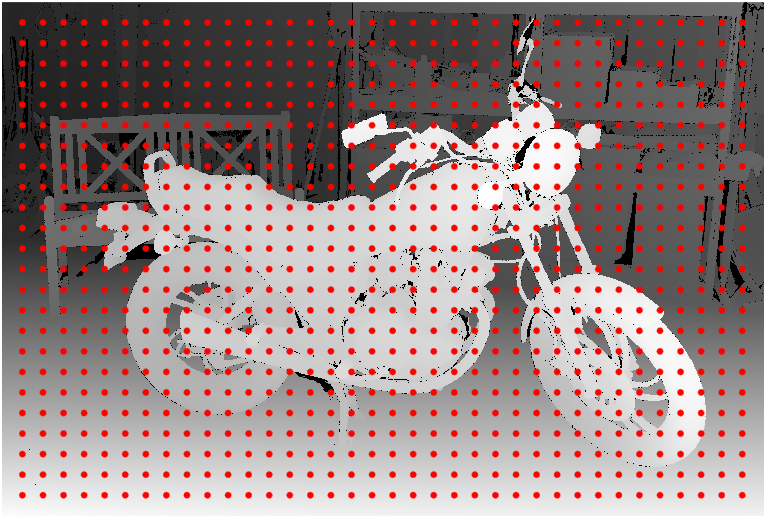
\includegraphics[width=0.4\textwidth]{images/disparity-plus-grid-test-left-01.png}
 		\label{fig:test-matlab-left-01}
}
	\subfigure[Right ground truth stereo test image overlapped by a simulated point grid]{
 		 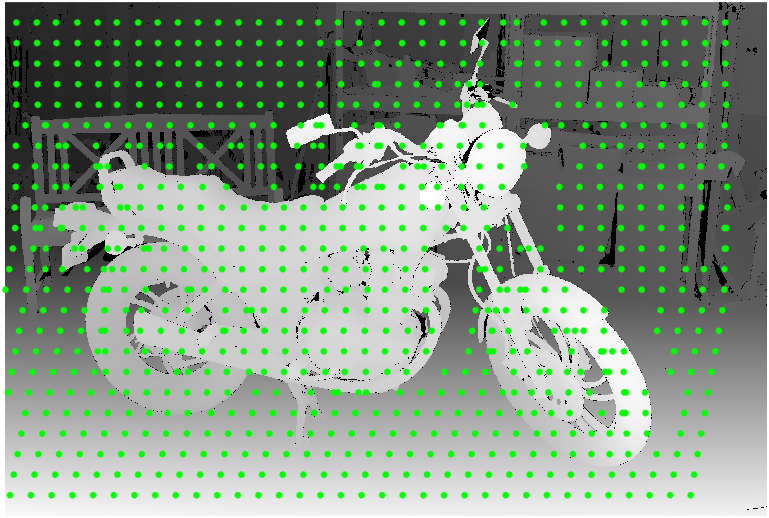
\includegraphics[width=0.4\textwidth]{images/disparity-plus-grid-test-right-01.png}
 		 \label{fig:test-matlab-right-01}
}
\caption{Ground truth images from the Middlebury dataset used for the initial testing phase}
\label{fig:test-matlab-01}
\end{figure}

As anticipated in Chapter~\ref{chapter:methods}, the first phase of the project can be mainly considered as a researching stage.
As a matter of fact, exploiting the stereo images from the Middlebury 2014 dataset, some tests have been performed to obtain an estimation of the feasibility of the conceived idea.\\
Therefore, as Figure~\ref{fig:test-matlab-01} displays, ground truth images have been initially used.
Thus, a point grid, similar to the one generated with the LadiMo device, has been simulated and overlapped to the input images.
In particular, as the difference between Figure~\ref{fig:test-matlab-left-01} and Figure~\ref{fig:test-matlab-right-01} illustrates, to have a reliable simulation of the 3D point cloud generated by the device, the only grid that was actually defined was the one over the principal image, i.e. the left one.
As a matter of fact, as defined in section~\ref{section:stereo-device}, the hardware exploited in the project is provided with only one laser projector.
Therefore, this allows to utilize the produce point cloud only over one image\footnote{Technically speaking the initial cloud of point created through the device can be independently related to both of the image, depending on which is used as the reference one, just applying the correct transformation between the laser system of reference and the reference one}.
After that, those input data, together with the grayscale stereo pair, have been employed in a stereo matching pipeline to recover a disparity map of the analysed scene.\\
In order to acquire useful baseline data regarding the practicability of the thought strategy, tests and analysis over the different areas of the main loop of the algorithm have been investigated.
Actually, this research has been performed with a precise method. \\
First of all the stages of a standard stereo matching method, as defined by Scharstein and Szeliski in \cite{Scharstein2001}, have been separately examined. 
Thus, in order to do this in a reasonable way, the literature regarding both standard and novel stereo matching algorithm has been studied and the main features of the designed algorithm checked out. 
As an example, if the matching cost phase is taken into account, different approaches are presented in the literature for evaluating the similarity among the image pixel values for the respective disparity levels. 
As a matter of fact, as introduced in Chapter~\ref{chapter:background}, the Hamming distance between corresponding pixels can be exploited to determine that measure. 
In relation to that, different algorithms exist to apply a transformation to the input images, making them available for an appropriate implementation of the aforementioned matching cost calculation.
For the actual tests carried out, local methods have been mainly analysed, being more appropriate for the type of data available and for the purposes of the designed strategy.\\
Therefore, as matching cost measures, simple operations have been initially taken into account, such as the sum of absolute differences and the sum of squared differences. 
Moreover, more accurate methods have been later evaluated, i.e. the Rank transform, and its improved version, the Complete Rank transform, broadly discussed in \cite{Demetz2013}.
Then, the Census transform and the Center-Symmetric Census transform proposed by Spangenberg et al. in~\cite{Spangenberg2013} have been investigated.
Considering all of those algorithm, it resulted that the most suitable methods are equivalently the rank and the census transform.
In fact, being these non-parametric transformations, they are not sensitive to changing in lightning inside the environment, thing that usually happen when managing real industrial areas. 
Considering that, at the end the Center-Symmetric Census transform has been chosen because of its reliability, which is comparable to the aforementioned methods, and for the fact that it uses a lower amount of bits to describe the single pixel value compared to the standard Census transform.\\
During this phase of testing, the decision was to run a single pipeline of an \textit{SGM-based} algorithm, whose aggregation cost phase would be based on the four orthogonal directions. 
Moreover, another operative choice was to use the whole image for the complete execution of the designed method.
Therefore, it was thought that, at least for this researching phase, it would be meaningless to define a hierarchical implementation of the code, where the image is initially downscaled and subsequently scaled up again in order to make the execution faster, as made by Hermann and Klette in their application of the Semi-Global Matching algorithm \cite{Hermann2013}.\\
At the end of this \textit{research} section of the project, the results did not show an exact path to follow. 
Specifically, the disparity image obtained was actually lower in accuracy compared to the method implemented in MATLAB by Eric Psota and available at the website of the Middlebury stereo dataset \footnote{\href{http://vision.middlebury.edu/stereo/submit3}{links Middlebury College Stereo}} and to the MATLAB built-in method \textit{disparitySGM}. 
Moreover, the developed implementation was quite slow, if correlated to the benchmark of most of the standard SGM-based methods. \\
However, some considerations should be proposed regarding that outcome. 
First of all, the algorithm designed runs iteratively, that is no parallel loop is coded to make the execution faster.  
This is, in fact, explained by the decision of being interested in the relative performance among the own designed methods. 
Furthermore, any sort of GPU enforcing was used. 
Hence, it was quite expected to not obtain good performance.
On the contrary, the thought strategy was evaluated as feasible and, additionally, the exploiting of proper initial data provided by the stereo camera would likely be an enhancement to the overall performance of the algorithm. \\

\section{Derivative based method implementation}
\label{section:derivative-based}

Verified the feasibility of the considered strategy, the project design shifted to the actual algorithm development. 
Therefore, exploiting the OpenCV libraries and using the images from the Middlebury 2014 dataset, the derivative based method started to be implemented in a C++ code. \\
In this initial phase of its designing, the simulated grid based on the ground truth images was still used as the method to obtain the input point cloud data.
As a matter of fact, the only practical advantage of employing such simulated data stands on the amount of noise that they contain.
As a matter of fact, an appropriate comment to that strategy would be that, once the real data from the device would be used, the result would be probably be worse in terms of overall accuracy. 
Anyway, at that initial stage of the algorithm development, the interest was focused on comparing the performance of the pure SGM-based and the derivative-based implementations. \\

\subsection{General features of the method and simulated grid specifications}
\label{subsection:general-feature-der-method}

\begin{figure}[t]
	\begin{center}
		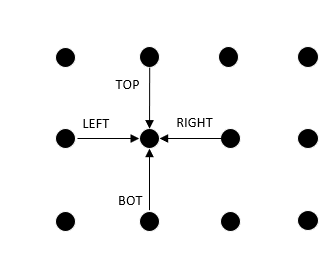
\includegraphics[width=.8\textwidth, height=7cm, keepaspectratio]{images/grid-subwindow-detail}
\caption{Detail of a point grid patch where a set of neighbouring points is highlighted}
\label{fig:grid-subpatch}
	\end{center}
\end{figure}

\begin{figure}[t]
	\begin{center}
		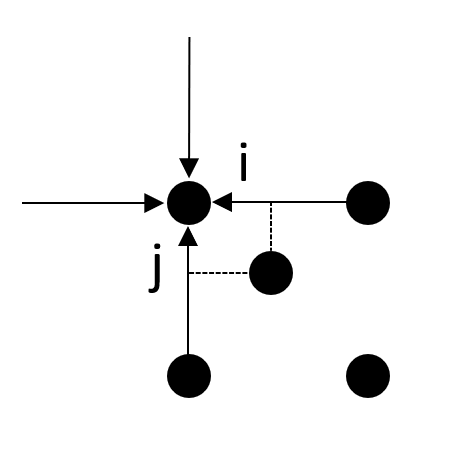
\includegraphics[width=.8\textwidth, height=7cm, keepaspectratio]{images/point-estimation-detail}
\caption{Detail of a point grid patch where the estimation of a new point at relative coordinates $i$ and $j$ is performed}
\label{fig:subpatch-estimation}
	\end{center}
\end{figure}

The so called derivative-based method, which arises to be both efficient and generally accurate, based its strength on the sparse point cloud gained through the structured light stereo camera.\\
The main features of that algorithm are now precisely described.
Moreover, attention is focused on the conventions utilized to define the main parts of the method and on the functions created for obtaining the 3D point estimations over the initial laser grid. 
Subsequently, some fundamental sections of the designed implementation are more broadly described, thus to provide to the reader a complete understanding of the work done. \\
For this reason, the analysis starts by considering a simulated grid of points, which was defined in the C++ code in order to initially mimic the real laser grid generated by the LadiMo device. 
This approach, as aforementioned, does not invalidate the outcome obtained through all the designing process of the method.
Instead, it is a reasonable strategy for achieving some initial temporary results, which can then provide a guidance to the following phases of the whole process.\\
Therefore, let us consider the entire point cloud as a regular grid where each point is defined by its coordinate in the space.
Additionally, it can be also thought that the corresponding 2D coordinates in the reference image plane can be easily retrieved using the camera matrices.
Hence, if a neighboring set of four points is taken into account, as highlighted by Figure~\ref{fig:grid-subpatch}, the local derivative vectors for all the considered coordinates can be easily calculated.
This estimation of the derivative is extremely useful for the following reasons.
First of all, they are, actually, exploited to generate the estimations inside each grid sub-region.
Moreover, they can be employed to evaluate if, inside the specific patch of points, there could be an edge of some shape. 
In this latter case, the magnitude of the Z component of the derivative vector will, in fact, be higher than a set threshold, which can be defined looking at the average values of the Z coordinate of the grid points.\\
Therefore, explaining the project design procedure implemented, it can be summarized as follows.
Initially, for each one of the points in the grid the derivatives have been calculated with respect to its four neighbors, as the rows in Figure~\ref{fig:grid-subpatch} underline. 
This means that each point will have, then, four distinct set of local derivatives, conventionally defined as follows:
\begin{itemize}
	\item \textbf{from top:} derivative between the specific point and its top neighbor;
	\item \textbf{from boottom:} derivative between the specific point and its bottom neighbor;
	\item \textbf{from left:} derivative between the specific point and its left neighbor;
	\item \textbf{from right:} derivative between the specific point and its right neighbor.
\end{itemize}
In these definition a neighbor to a point is defined with the subsequent rule. 
Let us consider a point, which is classified through the grid coordinates $r$, along the row grid direction, and  $c$, along the column direction. 
Its neighboring points are, hence, identified by:
\begin{itemize}
	\item \textbf{top} neighbor: with coordinates $r - 1$ and $c$;
	\item \textbf{bottom} neighbor: with coordinates $r + 1$ and $c$;
	\item \textbf{left} neighbor: with coordinates $r$ and $c - 1$;
	\item \textbf{right} neighbor: with coordinates $r$ and $c + 1$;
\end{itemize}
Using that scheme the four derivatives estimated for each point will contain the difference between the actual point  \textbf{\textit{full location components}} and the ones of the relative neighbor regarding.
In the implemented code, the introduced \textbf{\textit{full location components}} are in the order: the $x$ and $y$ components of the point projected in the principal image plane, therefore they are measured in pixels, the $X$, $Y$ and $Z$ space coordinates of the point, in meters, and finally, $d$ is the disparity value, in pixel, related to the depth of the point, which can be evaluated through equation~\ref{eqn:disparity-depth}.\\
Therefore, let us now consider to estimate an unknown point inside a subregion of the whole grid, that was decided to be identified by 4 points, as Figure~\ref{fig:subpatch-estimation} displays.
The final 3D coordinates of the new point will be, at first, defined by four different estimations, each one related to the four corners of the grid subwindow, as follows.
\begin{subequations}
\label{eqn:point-patch-estimation}
	\begin{align}
		est_{TL} = TL + i \cdot der_{from-left} + j \cdot der_{from-top} \\
		est_{TR} = TR + (i-1) \cdot der_{from-right} + j \cdot der_{from-top} \\
		est_{BL} = BL + i \cdot der_{from-left} + (j-1) \cdot der_{from-bottom} \\
		est_{BR} = BR + (i-1) \cdot der_{from-right} + (j-1) \cdot der_{from-bottom}
	\end{align}
\end{subequations}
where $TL$, $TR$, $BL$ and $BR$ respectively point to the estimation done with respect to the top-left corner of the grid sub-window, the top-right corner, bottom-left and bottom-right corner. 
Then, $i$ and $j$ are the relative $x$ and $y$ coordinates of the estimated point, whose values range between 0 and 1.
Finally, in the notation employed, $der_{dir}$ stands for the different derivative vectors related to each corner point and visualized by the arrows in Figure~\ref{fig:subpatch-estimation}. \\
Once, these estimations are achieved exploiting the derivatives, as equations in~\ref{eqn:point-patch-estimation} define, the best evaluation is obtained by calculating each matching cost between the corresponding pixels between the stereo images. 
The matching cost is determined following the subsequent routine.\\
In relation do this, it should be reported that, due to the researching aspect of this project, lots of changing have been made to the code.
Therefore, to provide a clear explanation of the decisions made and the procedure followed, which, otherwise, could appear sometimes winding, all the relevant changing to the functions used are disclosed. 
Beside this brief comment about the created code, the best, among four, estimation of the new grid point is such evaluated.\\
The estimation provides the values of the 3D coordinates of the calculated point and its disparity.
The point location is, then, projected through the camera matrix to the reference image (usually the left image) pixel coordinates and the corresponding position in the support image is determined using the estimated disparity value. 
At this point the matching cost is computed as the absolute difference between the intensity values of the analysed pixels in the left and in the right image planes. 
However, this kind of measure appears to give weak results. 
As a matter of fact, the main problem was that, in some situations, the estimation labelled as the best one actually contained a value of disparity doubtful, if compared to the one of the point's closest neighbours.  
Moreover, this generally happened in textureless regions, where it is obviously more difficult to make accurate estimations.\\
To overcome this problem, a penalty value was added to each partial estimation. 
Moreover, that value was weighted linearly basing on the distance between the estimated point and the corresponding corner. 
In this manner, the estimation, related to the disparity and to the coordinate values of the closest corner, is most likely to be addressed as the best one.
Once the best estimation for each new point is calculated, the evaluated values of the 3D point coordinate are processed, applying a morphological filter, in order to remove undesired noise and smooth out the overall data. \\
The estimation procedure just described is not actually able to handle all kind of situations, concerning the provided input objects.
In fact, incorrect values used to be estimated in sub-regions affected by edge features, and thus occlusions. \\
Therefore, to correctly manage these situations, multiple cases have been defined, regarding the edge cases. 

\subsection{Edge cases and penalty values discussion}
\label{subsection:edge-cases-and-penalties}

At first, four main conditions have been distinguished. 
These comprise the possibility to do not have any type of edge inside a grid subregions, the existence of a vertical edge in the patch, an horizontal edge case and finally a so called \textit{undefined} case has been defined.\\
Therefore, in each one of these situations, the point estimation procedure differs slightly, so that the aforementioned linear penalty can be more wisely set.
Regarding this two distinct values of the penalty have been employed, a lower and a higher value.
In fact, because it is not efficiently possible to correctly estimate the position of the potential edge, the choice of the correct estimation has to be somehow driven by exploiting the linear penalties. \\
Moreover, to identify the correct type of edge, the derivatives have been exploited and, specifically, the magnitude of the $Z$ component of the vector. 
Basically, a general edge case, which is equivalent to the \textit{undefined} condition, is initially determined by computing the absolute difference between the $Z$ components of all the possible couples of corners, i.e. the $Z$ value of the local derivatives, and comparing that with a pre-determined threshold, which is related to the average depth value of the initial points of the grid. \\
Therefore, during the algorithm pipeline, the possibility of having an edge feature inside the specific patch is initially checked.
Then, if the depth values of the four corner are almost equivalent, this means that that are is actually planar.
Thus, in this situation, a fast interpolation method is run, so that the overall computation can be even faster.\\
On the contrary, if a vertical or an horizontal edge is found, the small and big penalties are used accordingly.
For example, if the edge is vertical, the small penalty will be multiplied to the relative $y$-coordinate of the estimated point, instead the big penalty will weight the $x$-coordinate.\\
Finally, for the undefined case, the penalty weight is equivalent in both directions, $x$ and $y$, and its magnitude ranges between the two previously defined penalties. \\
Those three different edge cases are the one initially tested. 
However, later appeared that a more meaningful strategy is based on the definition of two grater categories, which would comprise the cases described above.
These two bigger classes describe, thus, \textbf{soft} and \textbf{strong} edges. 
In fact, results of tests done with dataset images show that employing a single threshold for the depth difference and focusing only over the edge direction was not entirely correct. 
As a matter of fact, in a generic scene different types of objects exists. 
Therefore, adapting the edge analysis to the object distances, for example between the whole foreground and the background and between the multiple objects in the foreground, would give, as the final outcome, a smoother and more accurate dense 3D point cloud.


\subsection{Derivative computation and sanity check}
\label{subsection:derivative-computation}




\section{Semi-Global Matching based method implementation}
\label{section:sgm-based}

\section{OpenCV built-in Semi-Global Box Matching algorithm}
\label{section:opencv-sgm-method}

\section{Pre-processing testing and analysis}
\label{section:pre-processing-impl}

\subsection{Look-up table and point grid pre-processing}
\label{subsection:grid-preprocessing}


\section{Post-processing testing and analysis}
\label{section:post-processing-impl}

\section{Preparation to future improvements}
\label{section:intro-future-improv}
